\chapter{\texorpdfstring{Business Processes}{Business Processes}}
\label{ch:02}
\lecturemeta{Lezione 02 \quad\textbullet\quad 2026-07-03 \quad\textbullet\quad Roberto Bruni}{Weske, \emph{Business Process Management}, Ch.1 · van der Aalst, \emph{Workflow Management}, Ch.1}

Questa lezione introduce il \textbf{vocabolario di base} del corso. Non c'è ancora nessun formalismo: l'obiettivo è capire \emph{cosa} sono i processi di business, \emph{da dove} nasce l'esigenza di ragionare "per processi", e \emph{quali} sono gli elementi (attori, casi, procedure, task, risorse) che ricorreranno in tutto il resto. Fissiamo i termini preferiti, ammettendo però sinonimi in modo intercambiabile. La terminologia tecnica resta in inglese, così come compare sulle slide.

\section{\texorpdfstring{Orientamento al processo (process orientation)}{Orientamento al processo (process orientation)}}

\subsection{\texorpdfstring{Dai prodotti al lavoro}{Dai prodotti al lavoro}}

Il punto di partenza è quasi ovvio, ma è importante seguirlo perché è la radice di tutto. Per vivere abbiamo bisogno di \textbf{prodotti} (cibo, vestiti, casa, trasporti, salute) e, sempre più spesso, di \textbf{servizi}, cioè prodotti immateriali come l'approvazione di un credito, la conoscenza, l'intrattenimento. Qualunque prodotto, materiale o immateriale, è l'esito di un certo \textbf{work}: un task, una funzione, un incarico, spesso solo un tassello di un'attività più grande.

Nessuno però è capace di produrre da sé tutto ciò di cui ha bisogno. Per questo i prodotti vengono scambiati attraverso il \textbf{market}: la distribuzione in cambio di denaro. È proprio l'esistenza del mercato a far nascere una gran quantità di \emph{lavoro derivato} che altrimenti non esisterebbe — commercio, banche, pubblicità, logistica, assicurazioni, e-commerce e così via — oltre al lavoro puramente interno che serve solo a tenere in piedi l'organizzazione, senza contribuire direttamente a soddisfare un bisogno.

\subsection{\texorpdfstring{Le unità di lavoro e la nascita del Taylorismo}{Le unità di lavoro e la nascita del Taylorismo}}

Di fronte a questa mole di lavoro, le persone lo organizzano in \textbf{work units} specializzate: divisioni relativamente autonome, ciascuna capace di fare bene una gamma limitata di prodotti o servizi. L'orientamento al processo nasce da una revisione critica di \emph{come} organizzare queste unità, un modo introdotto da \textbf{Frederick Taylor} (1856–1915).

L'idea di Taylor è che, analizzando scientificamente il lavoro, si possa trovare "la" maniera migliore di eseguirlo (la \emph{one best way}, tramite lo studio dei tempi e dei movimenti) e che questa maniera vada poi imposta dall'alto. Ne segue una netta separazione tra chi \emph{pensa} il lavoro e chi lo \emph{esegue}.

\begin{boxdefinition}{Taylorismo}
Applicazione di una \textbf{functional breakdown} del lavoro complesso: lo si scompone in unità di piccolissima granularità, così che una forza lavoro \textbf{altamente specializzata} possa svolgerle in modo efficiente. La ricerca della \emph{"one best way"} passa dallo studio scientifico del lavoro (time and motion study) e comporta la separazione tra \textbf{lavoro mentale} (la pianificazione, affidata al management) e \textbf{lavoro manuale} (l'esecuzione, affidata agli operai).
\end{boxdefinition}

Questa spinta verso la specializzazione non è un fatto improvviso, ma il punto d'arrivo di una lunga traiettoria storica. La si può leggere lungo due dimensioni parallele: cosa il lavoratore \emph{tiene a fuoco} (il suo \textbf{focus}) e quanto è specializzato (le sue \textbf{capabilities}).

\begingroup\small
\begin{tabularx}{\linewidth}{>{\raggedright\arraybackslash}X>{\raggedright\arraybackslash}X>{\raggedright\arraybackslash}X}
\toprule
\textbf{Epoca} & \textbf{Worker's focus} & \textbf{Worker's capabilities} \\
\midrule
\textbf{Prehistoric times} & l'intero processo, per \emph{tutti} i prodotti & \emph{pure generalist} \\
\textbf{Ancient times} & l'intero processo, per \emph{un singolo} prodotto & \emph{intermediate specialist} \\
\textbf{Middle Ages $\rightarrow$ Industrial} & una \emph{singola parte} di un processo, per un singolo prodotto & \emph{pure specialist} \\
\bottomrule
\end{tabularx}
\endgroup

\emph{Fig. — "Road to Taylorism": scorrendo dalle epoche antiche a quella industriale, il lavoratore si restringe progressivamente a una porzione sempre più piccola del processo, diventando specialista puro.}

Il taylorismo ha funzionato benissimo nella manifattura e ha alimentato la rivoluzione industriale con le catene di montaggio. Ma ha un rovescio della medaglia che diventa evidente quando lo si applica fuori dalla fabbrica.

\begin{boxwarning}{Il pitfall del Taylorismo}
Scomporre il lavoro in tante attività minime impone molti \textbf{handover}, cioè passaggi di consegne da un lavoratore all'altro. Finché i prodotti si assemblavano in pochi passi semplici, questi passaggi non costavano quasi nulla e non richiedevano di sapere cosa fosse successo prima. Ma nelle organizzazioni che trattano \textbf{informazione e dati immateriali} i passi di un processo sono strettamente \textbf{correlati}: per svolgere un passo serve spesso conoscere lo stato dell'intero caso. Qui gli handover diventano un problema serio, perché ogni passaggio richiede di trasferire anche il contesto, cioè conoscenza.
\end{boxwarning}

A questo si aggiunge un costo umano. In una società complessa, un'iper-specializzazione fa perdere ai lavoratori la visione d'insieme (la \emph{big picture}): non capiscono più come il proprio pezzetto si inserisca nel tutto, e questo genera \textbf{alienazione}, con ricadute negative sulla produttività (e sulla vita delle persone). Far sapere a un dipendente per quale cliente sta lavorando è, non a caso, un modo semplice per aumentarne motivazione e resa.

\begin{boxtip}{L'idea chiave della prospettiva a processo}
La risposta a questi problemi è \textbf{ricombinare} più unità di lavoro a grana fine in unità più grandi, riducendo così il numero di handover. Il prezzo da pagare è che i lavoratori devono avere competenze più ampie: diventano \emph{knowledge worker} con una visione dell'obiettivo finale. A livello organizzativo, questo orientamento al processo si realizza al meglio con una \textbf{struttura a matrice} (che vedremo tra poco). Il punto centrale è che ragionare per processi non serve solo a \emph{elencare} le attività, ma soprattutto a \textbf{studiare e migliorare le connessioni} tra di esse.
\end{boxtip}

\section{\texorpdfstring{Strutture organizzative (organizational structures)}{Strutture organizzative (organizational structures)}}

Se ragioniamo per processi, dobbiamo chiederci come sono organizzate le persone che li eseguono. Una \textbf{struttura organizzativa} stabilisce come lavoro, autorità e responsabilità vengono ripartiti tra il personale. Il vincolo di fondo è che ogni \textbf{resource} sa svolgere solo certi task, e ogni task può essere svolto solo da certe risorse: un cassiere di banca, per esempio, non può concedere un mutuo. Descrivere un processo significa allora indicare tre cose — \emph{quali} task servono, in \emph{quale ordine}, e \emph{chi} li esegue — e il modo in cui si assegnano i work item alle risorse incide moltissimo su efficienza ed efficacia.

Le risorse si classificano secondo due criteri complementari: le \textbf{functions} (le competenze e proprietà funzionali di una risorsa) e i \textbf{roles} (la posizione nell'organizzazione, come l'appartenenza a un gruppo o a un'unità di lavoro). Una stessa risorsa può ricoprire più ruoli, anche contemporaneamente. Su questa base si distinguono tre forme tipiche di struttura.

\subsection{\texorpdfstring{Struttura a rete (network)}{Struttura a rete (network)}}

Nella struttura a \textbf{rete}, attori autonomi collaborano per fornire prodotti o servizi senza una gerarchia. Le relazioni sono orizzontali: aggregazioni ad-hoc, outsourcing, ingresso e uscita dinamici dei membri dal team. È la forma più flessibile e meno rigida.

\subsection{\texorpdfstring{Struttura gerarchica (hierarchical)}{Struttura gerarchica (hierarchical)}}

La struttura \textbf{gerarchica} è organizzata come un \textbf{albero}. Poiché la nozione di albero tornerà spesso nel corso, conviene richiamarla con precisione.

\begin{boxdefinition}{Tree}
Un albero è un \textbf{grafo} (vertici + archi) in cui due qualsiasi vertici sono connessi da \textbf{esattamente un cammino} — equivalentemente, un grafo \textbf{connesso e aciclico}. - \textbf{Leaf}: un vertice di grado 1 (una "foglia" con un solo collegamento). - \textbf{Rooted tree}: un albero in cui si distingue un vertice speciale, la \textbf{root}; da lì gli archi si orientano implicitamente allontanandosi dalla radice.
\end{boxdefinition}

Calata sull'organizzazione, questa struttura prende il nome di \textbf{organization chart} (organigramma): i nodi interni dell'albero sono ruoli o funzioni individuali, le foglie sono lo staff o i dipartimenti, e i rami rappresentano le relazioni di autorità (chi comanda chi).

\subsection{\texorpdfstring{Struttura a matrice (matrix)}{Struttura a matrice (matrix)}}

La struttura a \textbf{matrice} è quella che serve davvero all'orientamento al processo, perché tiene insieme due dimensioni contemporaneamente: quella \textbf{gerarchica} (le funzioni, stabili) e quella \textbf{funzionale-dinamica} (i processi/progetti in corso). Concretamente, si ha \textbf{una riga per ciascun processo}: ogni persona resta inquadrata nella gerarchia delle funzioni, ma può avere anche uno o più capi legati ai progetti, i \textbf{project leader}.

\begin{figure}[!htb]
\centering
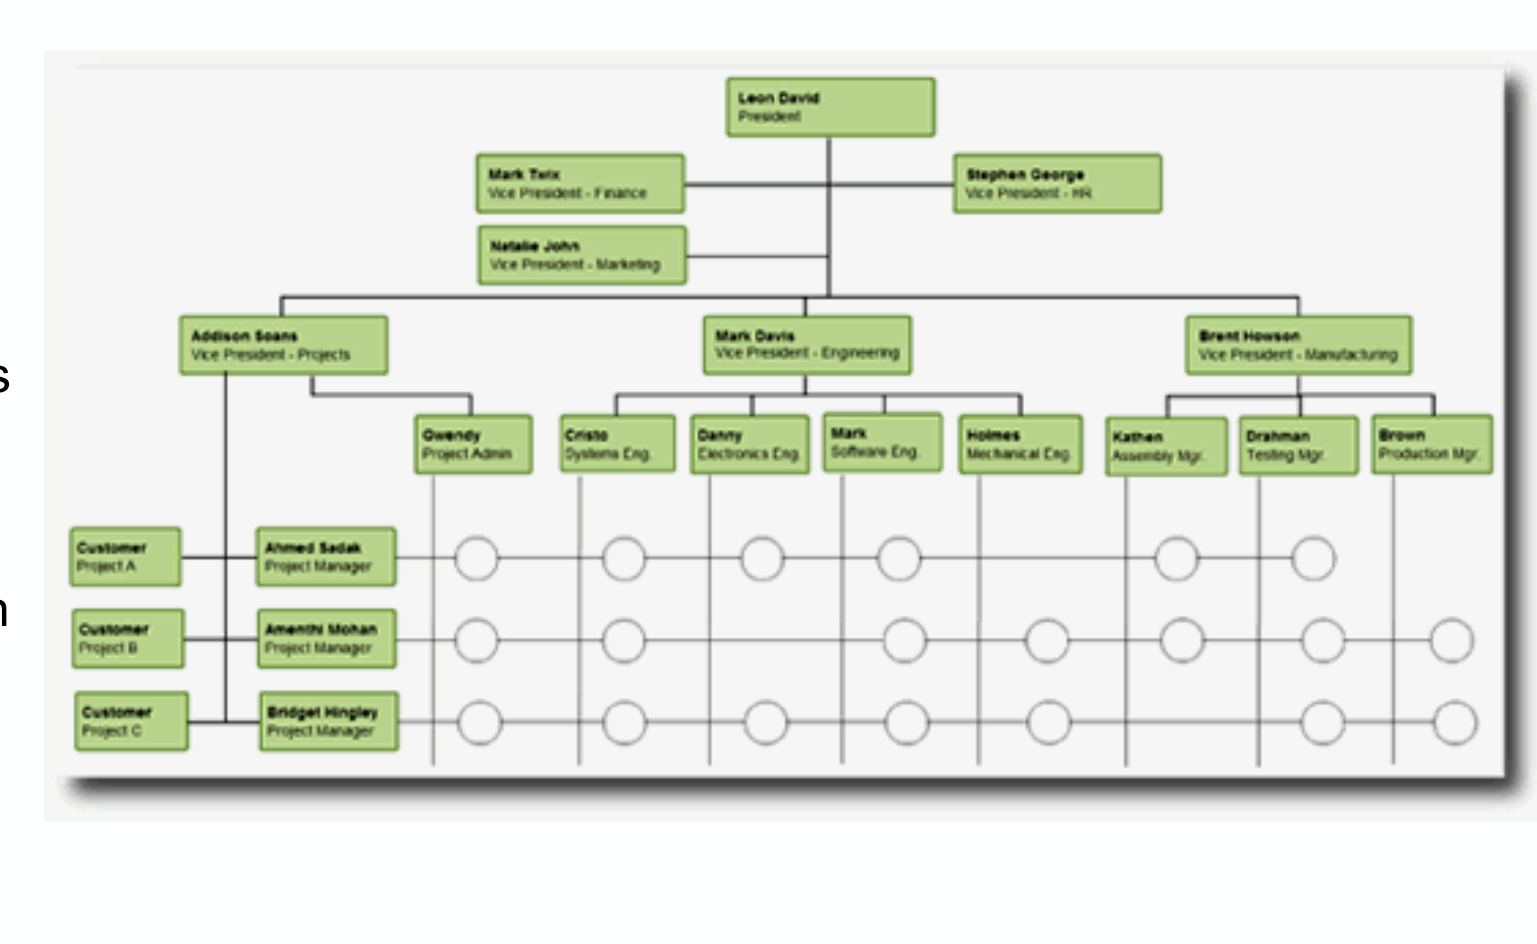
\includegraphics[width=0.53\linewidth,height=0.34\textheight,keepaspectratio]{images/02-business-processes_p21_matrix.png}
\caption{Struttura a matrice. Verticalmente scorre la gerarchia funzionale (President $\rightarrow$ Vice President $\rightarrow$ ruoli operativi); orizzontalmente, ogni riga è un progetto/cliente gestito da un project manager. I pallini alle intersezioni sono le assegnazioni: un progetto "attraversa" in orizzontale più funzioni della gerarchia — è esattamente la cross-functionality che ci interessa.}
\end{figure}

\section{\texorpdfstring{Attori (actors): principal e contractor}{Attori (actors): principal e contractor}}

Passiamo da come è organizzato il lavoro a chi lo commissiona e chi lo esegue. Nella pratica, gran parte del lavoro di una persona le viene \textbf{assegnato o dato in outsourcing} da qualcun altro: i suoi \textbf{principal} (che possono essere individui, dipartimenti o intere aziende). I principal si presentano in due forme, il \textbf{boss} e il \textbf{customer}, spesso collegate tra loro: un boss assegna un compito che a sua volta serve a soddisfare un customer. Chi riceve il compito è il \textbf{contractor} (e può essere non solo una persona, ma anche una macchina o un software).

Tra principal e contractor si stabilisce un \textbf{contract} sul caso da svolgere (con scadenza, prezzo, ecc.), e può nascere un vero e proprio \textbf{protocollo di comunicazione} per scambiarsi informazioni. Un dettaglio importante è che un attore non è per forza \emph{solo} principal o \emph{solo} contractor: può essere \textbf{entrambi allo stesso tempo}, perché un contractor può ri-delegare a terzi parte del lavoro ricevuto.

Il protocollo di comunicazione tra i due si legge come una sequenza di messaggi che vanno avanti e indietro:

\begin{center}
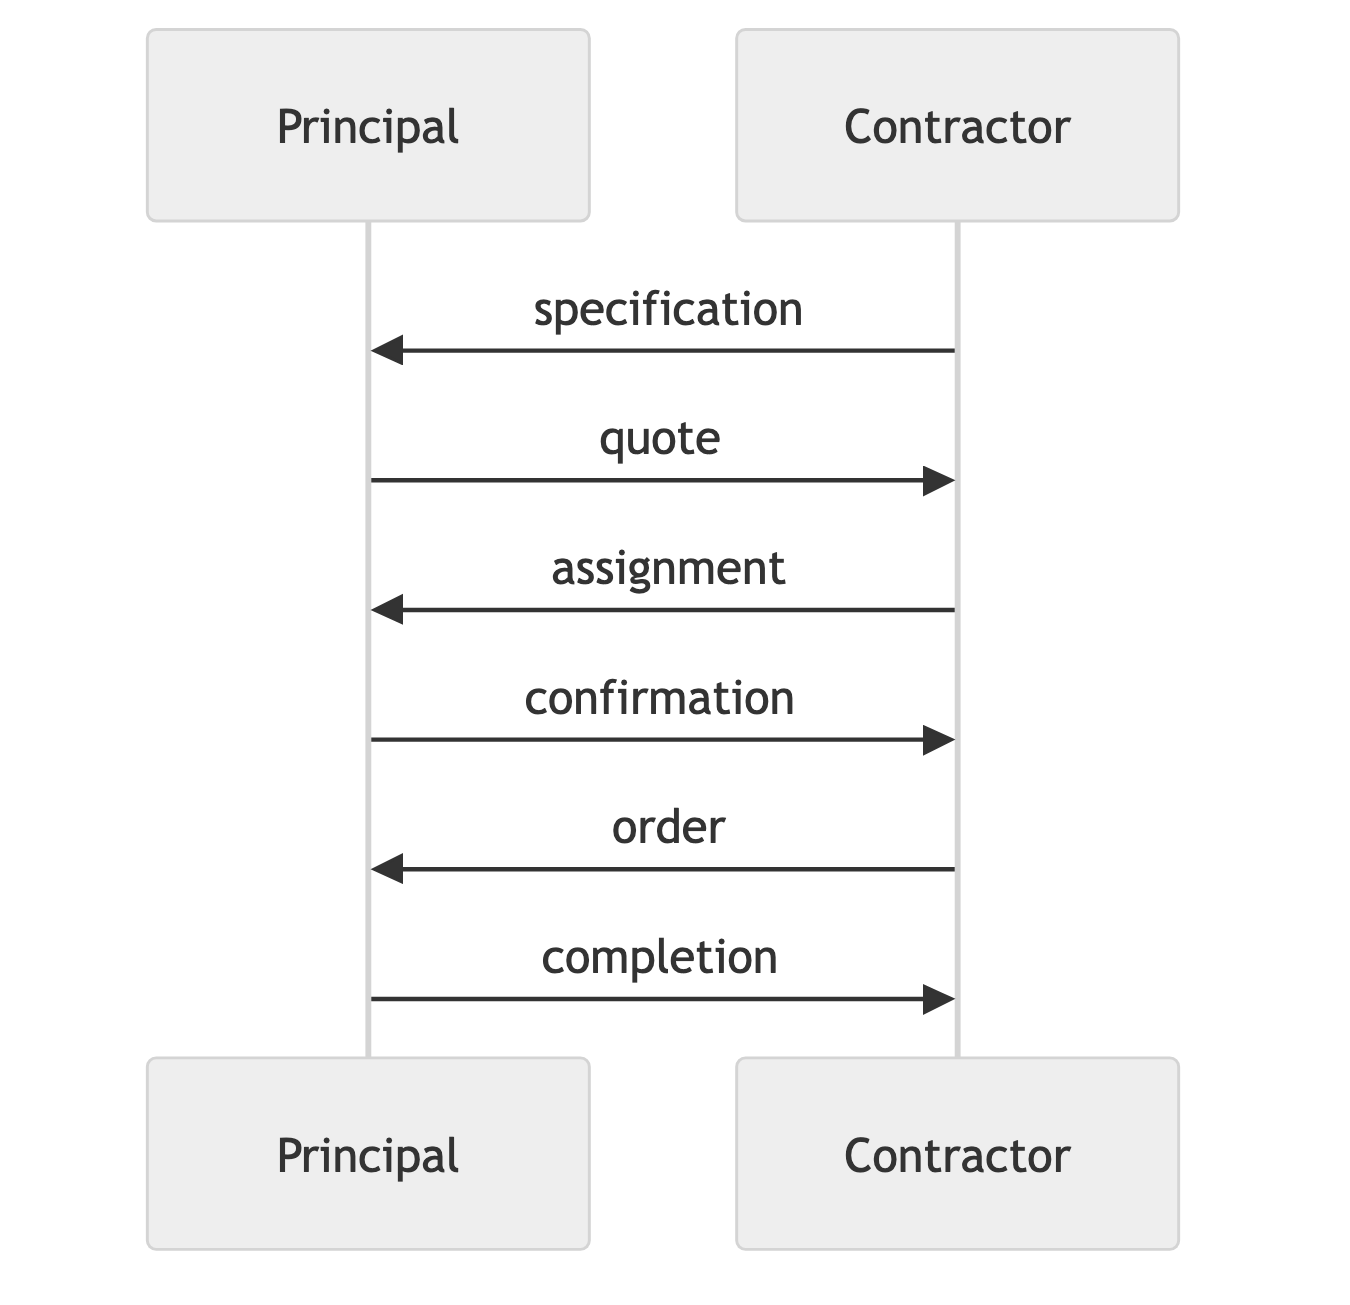
\includegraphics[width=0.74\linewidth,height=0.32\textheight,keepaspectratio]{images/mermaid/02_1.png}
\end{center}

E proprio perché un contractor può fare da principal verso altri, i contratti si concatenano in un \textbf{contract tree}. L'esempio classico è un trasporto complessivo che viene scomposto in sotto-trasporti affidati a contractor diversi:

\begin{center}
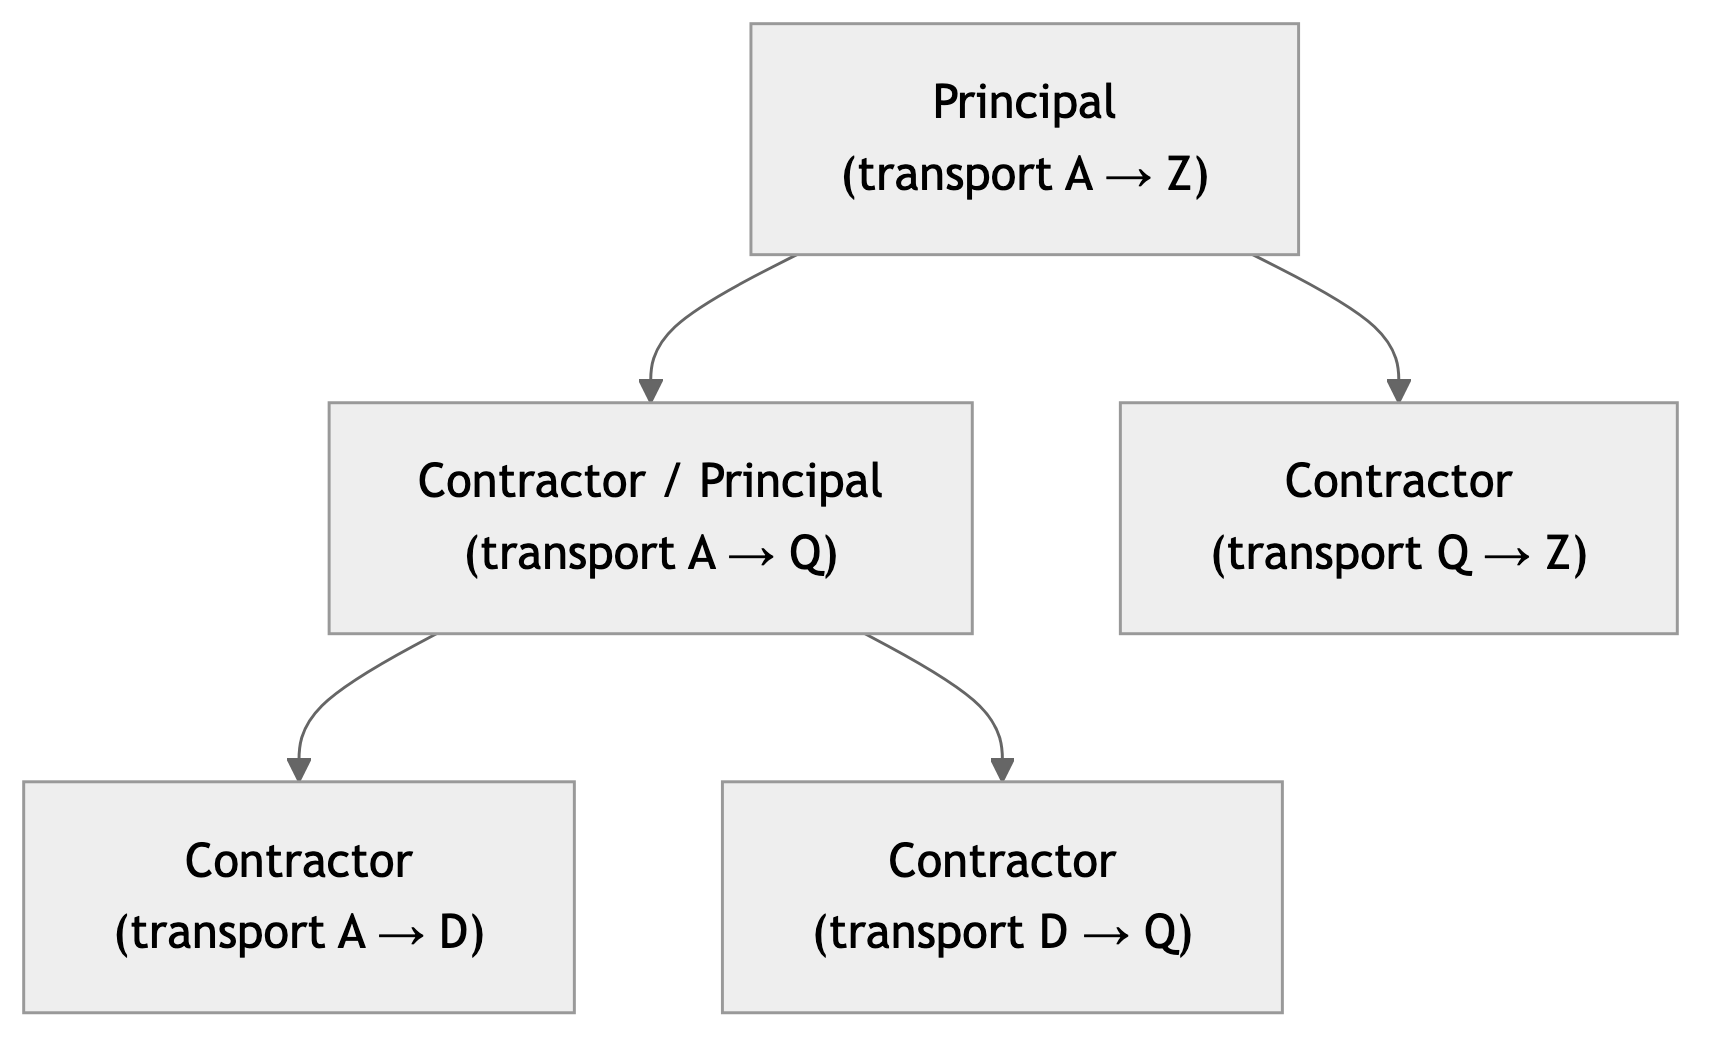
\includegraphics[width=0.74\linewidth,height=0.32\textheight,keepaspectratio]{images/mermaid/02_2.png}
\end{center}

Ogni nodo dell'albero è insieme il contractor di chi sta sopra e il principal di chi sta sotto: la delega si propaga verso il basso.

\section{\texorpdfstring{Casi, procedure, task, risorse, attività}{Casi, procedure, task, risorse, attività}}

Arriviamo ai mattoni concettuali con cui descriveremo qualunque processo. Sono cinque termini che è facile confondere, quindi conviene fissarli bene, uno per uno, cogliendo le relazioni tra loro.

\begin{boxdefinition}{Case}
Il \textbf{case} è l'oggetto concreto su cui si lavora. Spesso è una cosa tangibile che viene prodotta o modificata (una pagnotta, un mobile, una casa), ma può anche essere astratto (una causa legale, un sinistro assicurativo, dei dati digitali). Ogni caso ha un \textbf{inizio} e una \textbf{fine}, è \textbf{distinguibile} da ogni altro caso ed è di natura \textbf{discreta}. \emph{Sinonimi: work, job, product, service, item.}
\end{boxdefinition}

\begin{boxdefinition}{Procedure}
La \textbf{procedure} descrive \emph{come} si lavora su un caso: quali \textbf{task} eseguire e quali \textbf{condizioni} determinano il loro ordine. Ogni caso viene trattato eseguendo una procedura. \emph{Sinonimi: process, project.}
\end{boxdefinition}

\begin{boxdefinition}{Task}
Un \textbf{task} è un'unità \textbf{logica} di lavoro, che viene svolta come un tutt'uno indivisibile.
\end{boxdefinition}

\begin{boxdefinition}{Resource}
Una \textbf{resource} è il nome generico per una persona, una macchina, o un gruppo di persone/macchine \textbf{responsabile} di un task.
\end{boxdefinition}

\begin{boxdefinition}{Activity}
Un'\textbf{activity} è l'\textbf{esecuzione} effettiva di un task da parte di una risorsa. Ecco la distinzione sottile: una procedura è lo schema, l'attività è ciò che accade davvero. Casi diversi possono seguire la stessa procedura, ma comportare attività differenti a seconda dei loro attributi — un sinistro può richiedere obiezioni e un altro no, pur seguendo la stessa procedura.
\end{boxdefinition}

Il collante che tiene insieme questi concetti è la \textbf{knowledge}. Alcuni task li svolge un computer senza alcun intervento umano; altri richiedono intelligenza umana, cioè un giudizio o una decisione (un impiegato di banca che valuta una richiesta di prestito) e quindi conoscenza: esperienza pregressa, linee guida aziendali, contesto del caso.

\subsection{\texorpdfstring{Cases vs procedures: l'economia di scala}{Cases vs procedures: l'economia di scala}}

C'è un'osservazione quantitativa che spiega molte scelte aziendali: in una qualsiasi azienda il numero di \textbf{procedure} è generalmente \textbf{finito e molto più piccolo} del numero di \textbf{casi} da gestire. È più facile confezionare cento gonne con lo stesso modello che cento gonne con cento modelli diversi — in altre parole, il pronto-moda costa meno del su-misura.

\begin{boxtip}{Economy of scale}
Il costo per caso \textbf{diminuisce} al crescere del numero di casi trattati. La strategia che ne deriva è tenere \textbf{poche procedure} e far sì che ciascuna gestisca \textbf{quanti più casi possibile}. La situazione ideale è un piccolo insieme di buone procedure, ognuna capace di trattare molti casi.
\end{boxtip}

Si potrebbe obiettare: e i sarti su misura, gli architetti che progettano ogni casa da zero, un caso per processo? In realtà anche loro sfruttano \textbf{approcci standard}. Il sarto, per esempio, segue sempre lo stesso schema — prende le misure, mostra alcuni modelli, modifica quello scelto, sceglie il tessuto, traccia il cartamodello — pur adattandolo al singolo cliente. L'osservazione generale, allora, è che \textbf{l'esecuzione di un task può dipendere fortemente dal caso}, senza per questo rinunciare a una procedura comune.

\section{\texorpdfstring{Cosa sono, in sostanza, i business process}{Cosa sono, in sostanza, i business process}}

Con questo vocabolario possiamo dire cosa sono davvero i processi di business. Ogni prodotto che un'azienda offre al mercato è l'esito di una serie di task; i \textbf{business process} riguardano la \textbf{comprensione, correlazione, organizzazione e miglioramento} di quelle attività. Su questa idea si innesta il \textbf{Business Process Reengineering}: la convinzione che una riprogettazione \textbf{rapida e radicale} dei processi — e non solo miglioramenti graduali — possa essere la via al successo. Il cambiamento di prospettiva chiave è lo spostamento del focus dal \textbf{prodotto} (\emph{what}, cosa si fa) alla \textbf{logica di business} (\emph{how}, come il lavoro viene svolto).

\subsection{\texorpdfstring{Le radici del concetto (anni '90)}{Le radici del concetto (anni '90)}}

Il concetto di processo si è affinato attraverso alcune definizioni storiche, ciascuna delle quali mette a fuoco parole-chiave diverse. Metterle una accanto all'altra aiuta a cogliere le proprietà essenziali.

\begin{boxnote}{Le definizioni storiche di \emph{business process}}
\begin{itemize}
\item \textbf{Hammer \& Champy (1993)} — "una collezione di attività che prende uno o più input e crea un output \emph{di valore per il cliente}." Parole-chiave: \emph{collection, input, output.}
\item \textbf{Davenport (1993)} — "un insieme strutturato di attività per produrre un output specifico per un mercato particolare; uno specifico ordinamento di attività nel tempo e nello spazio, con un inizio e una fine." Parole-chiave: \emph{structure, ordering, time, space, begin, end.}
\item \textbf{Johansson et al. (1993)} — "un insieme di attività \emph{collegate} che prendono un input e lo trasformano in un output"; e la trasformazione deve \textbf{aggiungere valore}. Parole-chiave: \emph{recipient, linked.}
\item \textbf{Rummler \& Brache (1995)} — distingue i \textbf{production processes} (il cui output è ricevuto dal cliente esterno) dagli altri, invisibili all'esterno ma essenziali per gestire l'azienda.
\end{itemize}
\end{boxnote}

Mettendo insieme queste definizioni, un processo ha alcune \textbf{proprietà ricorrenti}, che vale la pena enunciare distintamente:

\begin{itemize}
\item è una \textbf{collection}: raggruppa un insieme di task;
\item ha \textbf{definability}: confini, input e output chiaramente definiti;
\item è \textbf{ordered}: i suoi task sono ordinati secondo la loro posizione nel tempo e nello spazio;
\item ha un \textbf{customer / recipient}: il suo output è destinato a qualcuno;
\item è \textbf{linked}: le attività sono collegate lungo una catena a valore aggiunto, cioè in un ordine di esecuzione.
\end{itemize}

Quest'ultimo punto — l'ordinamento tra i task — merita un formalismo, perché è il cuore di ciò che modelleremo. L'ordine parziale tra i task si esprime con una \textbf{relazione di precedenza} $\prec$: fissato un insieme di task e dei vincoli, solo alcune sequenze di esecuzione (\textbf{execution trace}) rispettano quei vincoli e sono quindi valide.

\begin{boxexample}{Precedenza ed execution trace}
Prendiamo l'insieme di task $S = \{a, b, c, d, e, f\}$ con la relazione di precedenza:

\[
\begin{aligned}
a &\prec b \prec d \prec f \\[4pt]
a &\prec c \prec e \prec f \\[4pt]
c &\prec d
\end{aligned}
\]

che si legge come il grafo di precedenza:

\begin{center}
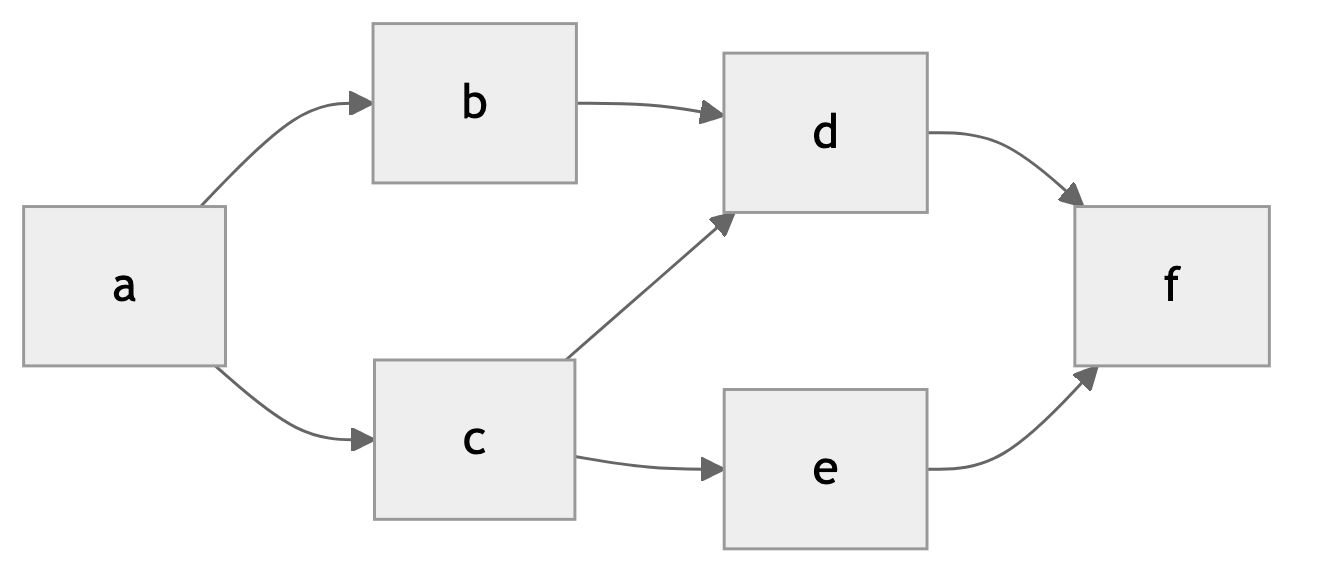
\includegraphics[width=0.74\linewidth,height=0.32\textheight,keepaspectratio]{images/mermaid/02_3.png}
\end{center}

Una trace è \textbf{valida} se rispetta \emph{tutti} i vincoli $\prec$. Per esempio \texttt{a b c d e f} e \texttt{a c b e d f} sono valide; invece \texttt{a b d c e f} \textbf{non} lo è, perché mette $d$ prima di $c$ violando il vincolo $c \prec d$. Il grafo, in fondo, dice solo quali passi devono precedere quali altri: qualunque ordine compatibile con tutte le frecce è ammesso.
\end{boxexample}

\subsection{\texorpdfstring{Ownership e cross-functionality}{Ownership e cross-functionality}}

Un processo ben strutturato ha un vantaggio pratico: è \textbf{misurabile} lungo diverse dimensioni (costo, tempo, qualità dell'output, soddisfazione del cliente). E poiché è misurabile, migliorarlo ha un significato preciso: ridurre il costo o aumentare la soddisfazione \emph{è} migliorare il processo. Perché ciò funzioni servono due condizioni.

La prima è l'\textbf{ownership}: deve esistere \textbf{un} responsabile della performance e del miglioramento continuo del processo. Durante i cambiamenti radicali, questa ownership deve addirittura prevalere sulle altre strutture organizzative, altrimenti il responsabile non avrebbe il potere di imporre modifiche che vanno contro l'organigramma esistente.

La seconda è la consapevolezza della \textbf{cross-functionality}: un processo tipicamente \textbf{attraversa più funzioni}, dentro e attraverso la struttura organizzativa. Entra un input, il processo tocca funzioni diverse dell'azienda, e ne esce un output diretto al customer — proprio come si vedeva orizzontalmente nell'organigramma a matrice.

\subsection{\texorpdfstring{Primary, secondary e tertiary process}{Primary, secondary e tertiary process}}

Infine, i processi si classificano secondo il loro ruolo nell'azienda, in tre livelli:

\begin{itemize}
\item \textbf{Primary process} (processi di produzione): producono i prodotti dell'azienda, sono orientati al cliente e generano il reddito. Esempi: acquisto di materie prime, vendita di servizi, progettazione e ingegnerizzazione, distribuzione.
\item \textbf{Secondary process} (processi di supporto): sostengono quelli primari senza generare reddito diretto. Esempi: manutenzione dei macchinari, gestione del personale (selezione, formazione, buste paga), amministrazione finanziaria, marketing.
\item \textbf{Tertiary process} (processi manageriali): dirigono e coordinano primari e secondari, fissando obiettivi, allocando risorse e stabilendo le precondizioni per i manager degli altri processi. Esempio: la gestione dei contratti con finanziatori e stakeholder.
\end{itemize}

\section{\texorpdfstring{Verso una notazione standard}{Verso una notazione standard}}

Resta un'ultima domanda, che fa da ponte con la lezione successiva: perché serve \textbf{standardizzare} il modo di descrivere i processi? Perché ci sono due mondi che devono parlarsi — gli \textbf{aspetti organizzativi di business} da un lato e l'\textbf{information technology} dall'altro — e un linguaggio comune è l'unico modo per farlo. I \textbf{linguaggi visuali} sono ottimi allo scopo: sono intuitivi, universali, immediati, non tecnici e richiedono poca conoscenza pregressa. La scelta più naturale, per rappresentare processi, è quella di \textbf{nodi e frecce} (i grafi orientati).

\begin{boxdefinition}{Notazione standard (diagrammatica)}
Un insieme \textbf{piccolo e predefinito} di forme e linee, ciascuna con un significato \textbf{non ambiguo}. Colori, bordi e simboli diversi possono assegnare significati o informazioni aggiuntive (per esempio, frecce diverse per dipendenze diverse). I concetti che una tale notazione deve saper esprimere sono: \emph{start, end, task, link, order, ownership, responsibility.}
\end{boxdefinition}

È esattamente questo il tema della prossima lezione, dove vedremo come questi concetti diventano simboli grafici precisi — e scopriremo che "nodi e frecce" da soli non bastano. $\rightarrow$ \hyperref[ch:03]{03 — Visual Notation}